\documentclass[twoside,a4paper]{refart}
\usepackage{makeidx}
\usepackage{ifthen}
\usepackage{graphicx}
\usepackage{float}
\usepackage[portuguese]{babel}

\def\bs{\char'134 } % backslash in \tt font.
\newcommand{\ie}{i.\,e.,}
\newcommand{\eg}{e.\,g..}
\DeclareRobustCommand\cs[1]{\texttt{\char`\\#1}}

\title{Manual de Operação Linux CNC}
\author{Grupo 2 - Projeto de Máquina PMR3411 - 2024 \\
Vinicios de Andrade Cardozo \\
Gabriel Silva de Carvalho  \\
Douglas \\
Versão 1}

\date{}
\emergencystretch1em  %

\pagestyle{myfootings}
\markboth{Manual de operação do torno}%
         {Manual de operação do torno}

\makeindex 

\setcounter{tocdepth}{2}

\begin{document}

\maketitle

\begin{abstract}
Por meio deste texto vamos apresentar de maneira resumida a operação básica do torno controlado pelo Linux CNC, levando em conta peculiaridades presentes no controlador em relação a outras opções mais comuns e também as advindas de escolhas que ficaram a cargo do grupo de programação do projeto.
\end{abstract}

\tableofcontents

\newpage


%%%%%%%%%%%%%%%%%%%%%%%%%%%%%%%%%%%%%%%%%%%%%%%%%%%%%%%%%%%%%%%%%%%%

\section{Procedimentos inicias}

Aqui trataremos dos passos iniciais para começar a operar a máquina, ou seja, passos a serem realizados antes mesmo que o botão de ligar seja ativado na interface gráfica do aplicativo do LinuxCNC. 

\subsection{Inicialização e login}

Antes de ligar o computador é recomendável verificar que o Joystick esteja acoplado em uma entrada USB, uma vez que o LinuxCNC pode apresentar problemas de varredura de periféricos, ou seja, ele pode não detectar dispositivos conectados após sua inicialização (apesar de que esse problema nunca se apresentou para o caso de pendrives).

O próximo passo é conectar a caixa de controle a \textbf{uma tomada de 220V} (na sala de laboratório essas tomadas tem cor vermelha), e então ligar a caixa. Note que a caixa deve ser ligada antes de se ligar o computador pelo mesmo problema de varredura anteriormente citado.

Com os passos anteriores feitos, o computador pode ser ligado. Para acessá-lo basta que se entre com o login: \textbf{alunopmr} e a senha: \textbf{pmrcnc}. 

A última coisa a se fazer antes de se abrir o aplicativo do LinuxCNC é abrir um terminal e executar o comando: \textbf{qjoypad} para inicializar a aplicação que irá receber os inputs do Joystick e convertê-los para comandos de teclado que o LinuxCNC compreende. 

\subsection{Preparação para carregar um código G}
Abra o aplicativo do LinuxCNC, selecionando a configuração correta para o torno que será utilizado. Abaixo, alguns métodos para se selecionar a configuração correta:

\begin{figure}[H]
    \begin{center}
        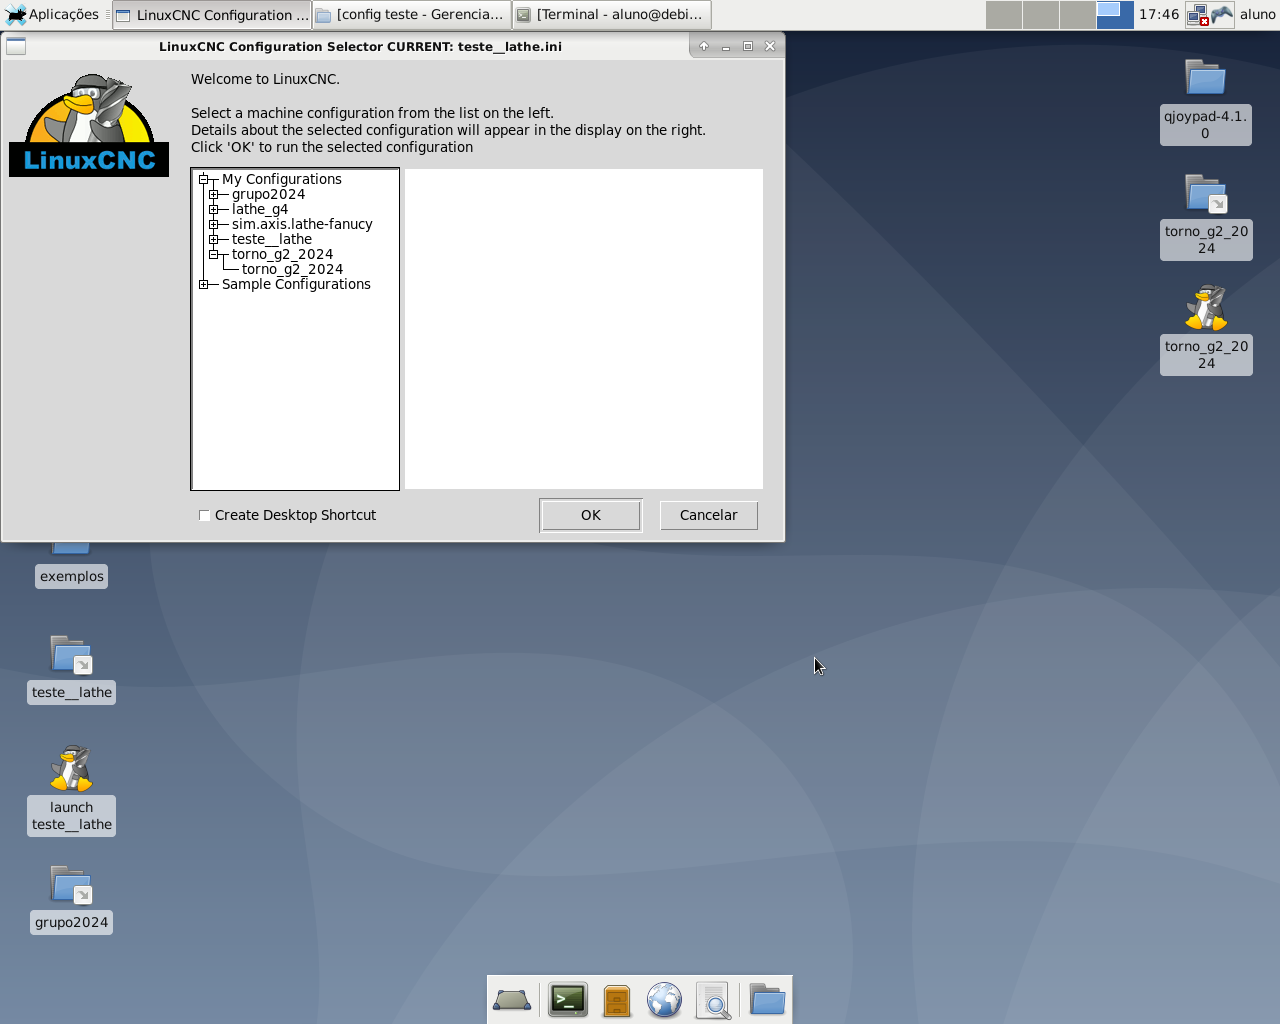
\includegraphics[width=0.95\textwidth]{imagens/Abertura_do_linux_CNC.png}
    \end{center}
    \caption{}\label{abrircncpiorjeito}
\end{figure}

Já com o aplicativo do LinuxCNC aberto, procure pelo botão vermelho de ligar no canto superior esquerdo da interface gráfica ou simplesmente utilize o botão "start" do Joystick, isso irá efetivamente ligar a máquina. 
Com o controle manual (Joystick ou teclado) leve o torno para uma posição segura e então faça o \textbf{homing} dos eixos X e Z.

\begin{figure}[H]
    \begin{center}
        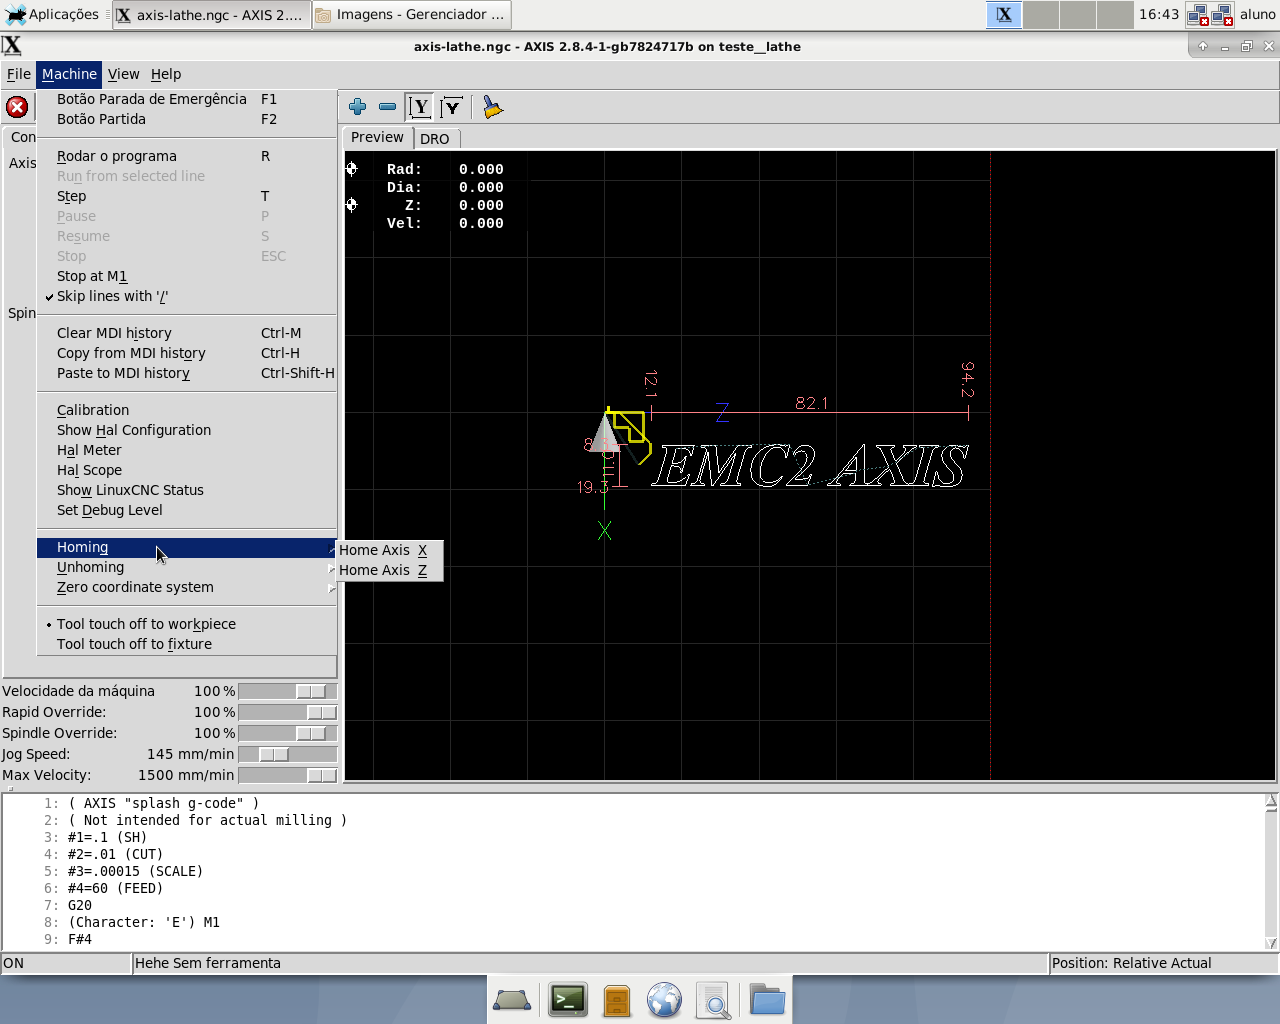
\includegraphics[width=0.95\textwidth]{imagens/referenciamento_linux_CNC.png}
    \end{center}
    \caption{}\label{homing}
\end{figure}


Para códigos G que descrevem diâmetros ao invés de raios (ou seja, códigos G usuais) é preciso que se ative o modo de diâmetro usando o comando G7 no MDI.

    Abra o código G da peça que você deseja produzir. Se houver algum erro na abertura modificações no código podem ser necessárias.

\begin{figure}[H]
    \begin{center}
        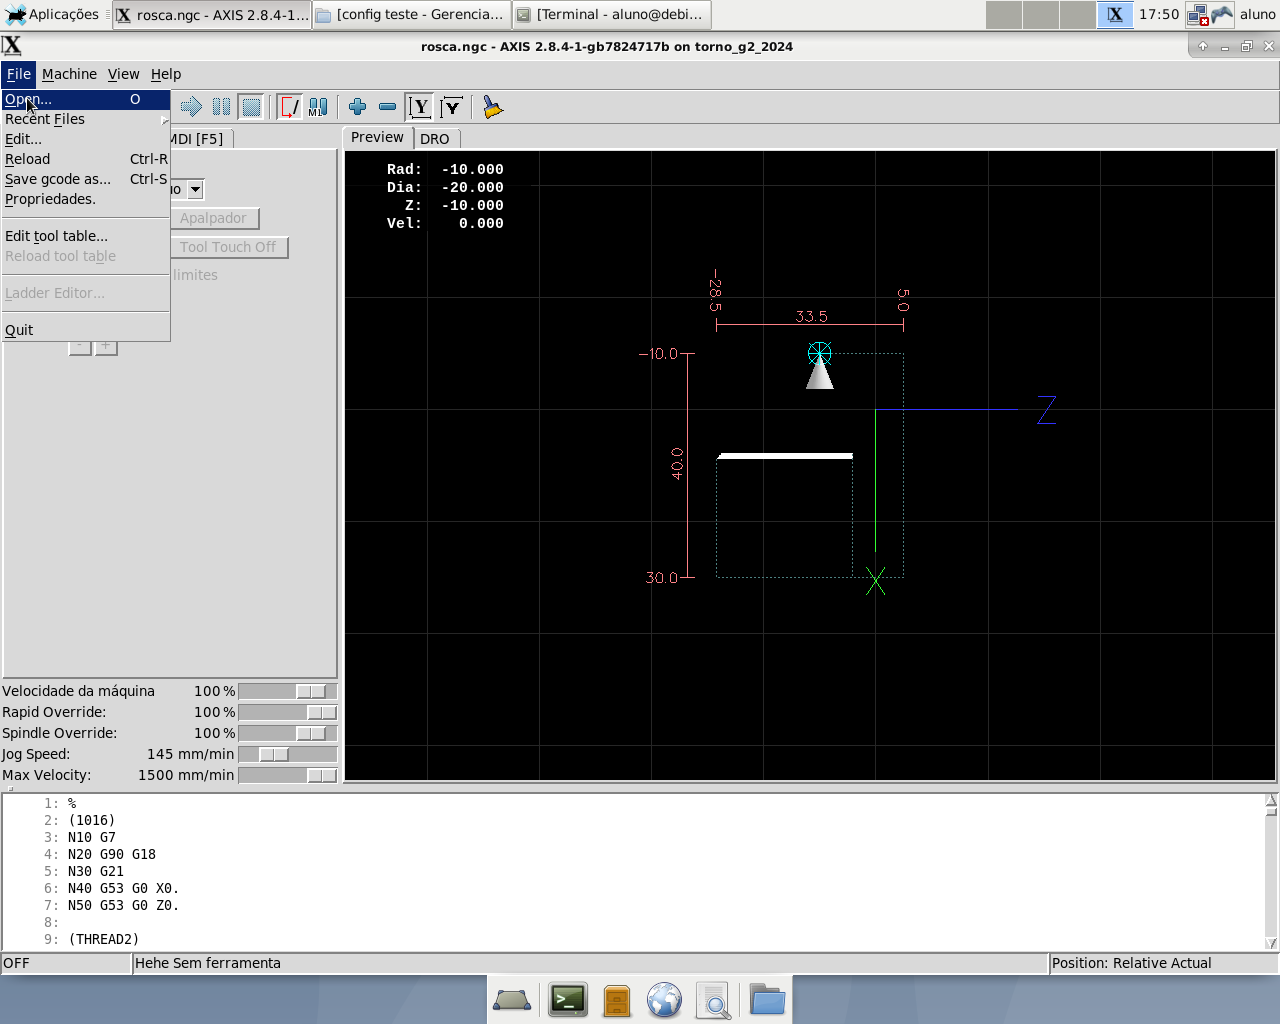
\includegraphics[width=0.95\textwidth]{imagens/Selecao_do_programa2.png}
    \end{center}
    \caption{}\label{progselec}
\end{figure}

\begin{figure}[H]
    \begin{center}
        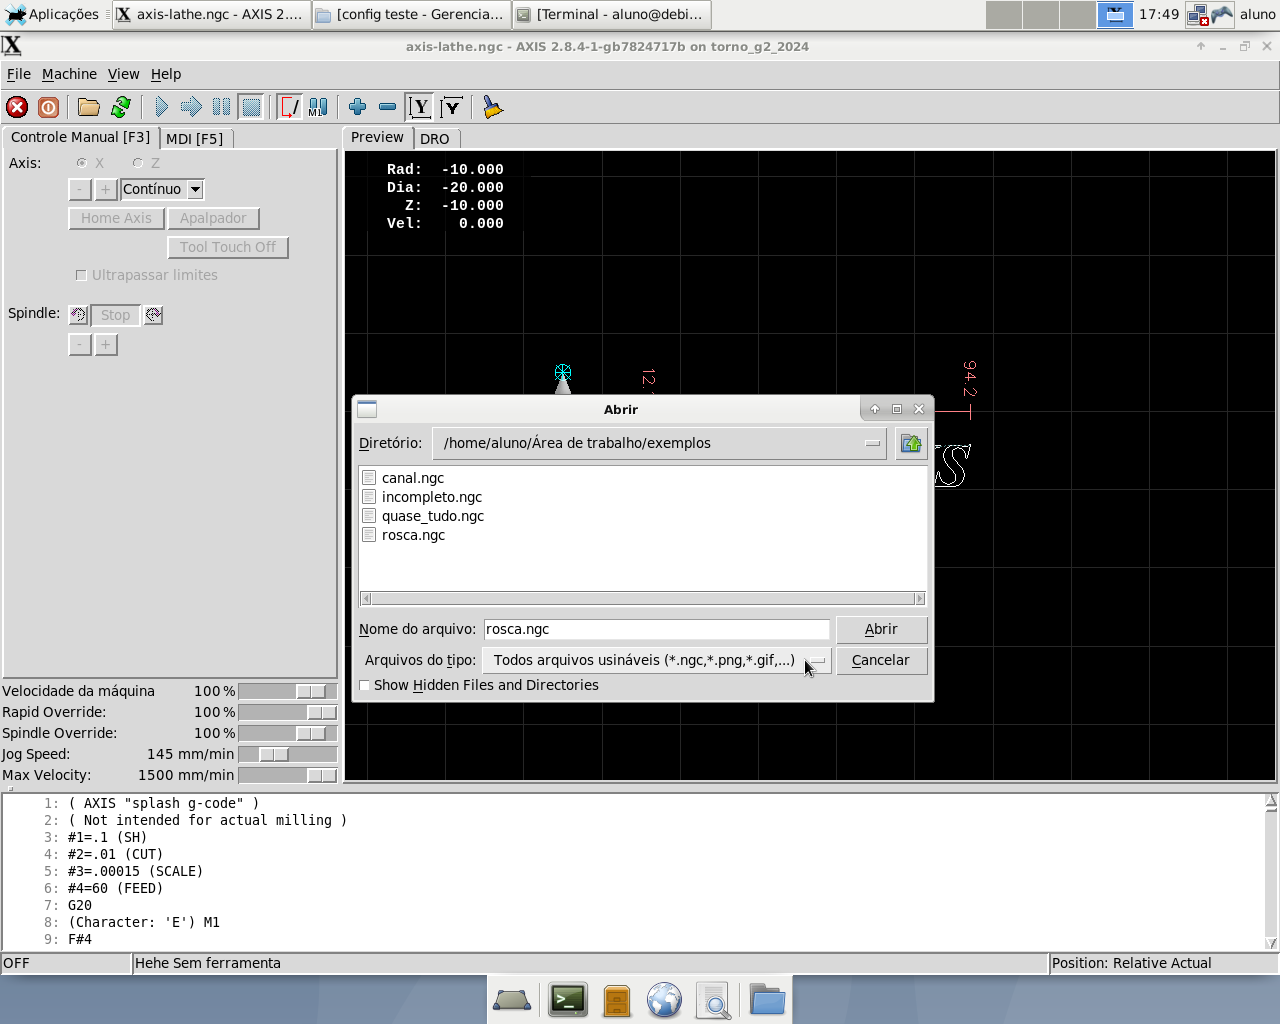
\includegraphics[width=0.95\textwidth]{imagens/Selecao_do_programa.png}
    \end{center}
    \caption{}\label{progselec2}
\end{figure}

\section{Controles}

O controle manual da máquina é feito através de comandos de teclado que podem ser consultados através da referência rápida do menu "help" do aplicativo do LinuxCNC. Através do uso do qjoypad esse controle pode ser feito através de um Joystick, sendo essa a forma que vai ser avaliada no dia da apresentação final e portanto a forma recomendada. 

Nessa seção são listados todos os comandos programados para funcionar no Joystick, de modo a melhorar a experiência de qualquer usuário seguindo os passos das próximas seções desse manual. 

\begin{itemize}
    \item Direita 
    \item Esquerda
    \item Cima
    \item Baixo
    \item Aumentar velocidade 
    \item Diminuir velocidade
    \item Selecionar eixo X
    \item Selecionar eixo Z
    \item Homing do eixo selecionado
\end{itemize}

\section{Definição do zero peça}

O zero peça é a referência relativa ao zero máquina que passamos ao LinuxCNC para que o mesmo saiba em que coordenadas o material bruto que deve ser torneado está localizado. Podem ser definidos, através de diferentes códigos G, diversos planos de corte, sendo o P0 o plano padrão, em coordenadas absolutas definidas na etapa de homing da máquina.

Para definir o zero peça devemos definir um novo plano de corte utilizando a função de \textbf{apalpador} localizada ao lado do botão de homing. Apesar de não ser obrigatório, dê preferência a definir o zero peça usando o plano definido por G54. Abaixo temos uma imagem da função de apalpador sendo utilizada.

\begin{figure}[H]
    \begin{center}
        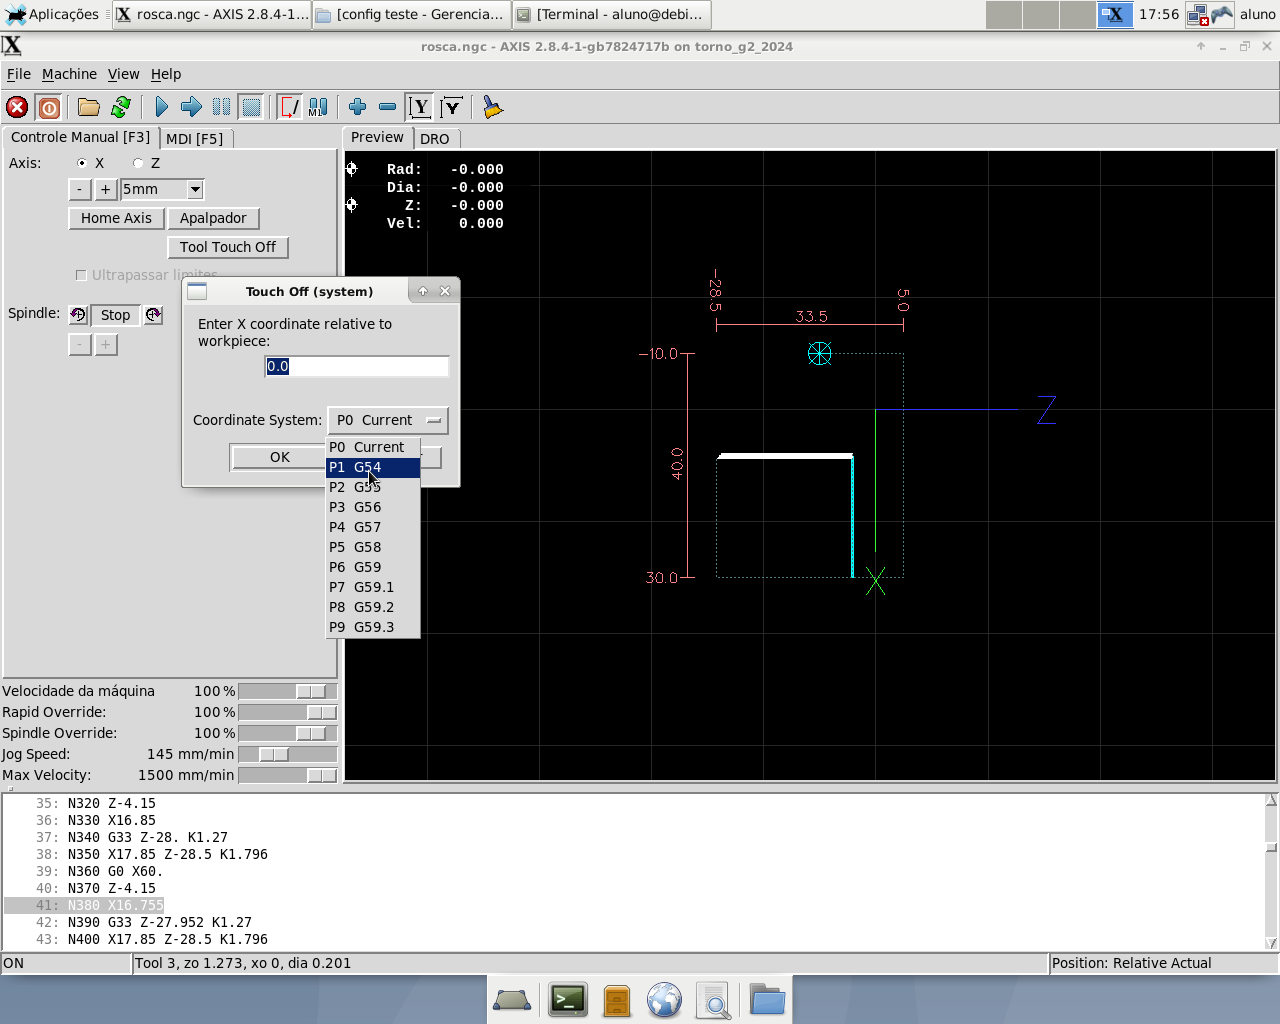
\includegraphics[width=0.95\textwidth]{imagens/Definicao_do_zero_peca_g54.png}
    \end{center}
    \caption{}\label{G54}
\end{figure}


A seguir, uma breve descrição do como usar a função do apalpador para definir o zero peça em cada um dos eixos.

\subsection{Eixo Z}

Leve a ferramenta até a face do tarugo e encoste nela com \textbf{cuidado}, utilizando de preferência o d-pad do Joystick (o teclado também funciona, mas utilizar o Joystick é parte da avaliação). 

Confira se o eixo Z aparece selecionado antes de prosseguir, se não estiver selecione-o de um dos seguintes modos: clicando na opção com o mouse, mudando para o eixo Z usando o L2 do Joystick (recomendado) ou ainda usando o atalho de teclado Z (z maiúsculo).

Clique em apalpador, mantenha o offset em 0, selecione o plano de corte desejado (por favor use o G54 como o padrão para essa operação), clique em "OK". Isso deve mover a imagem da peça na tela, para a nova posição Z que você indicou através desse procedimento.

\attention Use o bom senso ao fazer esse procedimento, controlando a velocidade de aproximação usando os triggers superiores do controle para aumentar ou diminuir a velocidade (L1 diminui a velocidade e R1 aumenta). Consulte o slider na interface gráfica com o nome de "Jog speed" para ver a velocidade com a qual você está avançando (o slider pode ser usado para controlar essa velocidade também, mas novamente é recomendável o uso do Joystick). 

\attention Recomendamos velocidades de aproximação baixas (20 a 50 mm/s) quando prestes a encostar no tarugo de material.

\subsection{Eixo X}

Para esse eixo é preciso conhecer o diâmetro do tarugo que vai ser torneado. Idealmente deve-se fazer um passo manual de desbaste para garantir um diâmetro uniforme ao longo de todo comprimento do tarugo.

De pose dessa informação, leve a ferramenta até a lateral do tarugo e encoste nela com \textbf{cuidado}, utilizando de preferência o d-pad do Joystick (o teclado também funciona, mas utilizar o Joystick é parte da avaliação). 

Confira se o eixo X aparece selecionado antes de prosseguir, se não estiver selecione-o de um dos seguintes modos: clicando na opção com o mouse, mudando para o eixo X usando o R2 do Joystick (recomendado) ou ainda usando o atalho de teclado X (x maiúsculo).

Clique em apalpador, o offset que você deve informar é o diâmetro (assumindo que G7 foi ativado, se não, o raio) do tarugo que você está prestes a tornear, selecione o plano de corte desejado (por favor use o G54 como o padrão para essa operação), clique em "OK". Isso deve mover a imagem da peça na tela, para a nova posição X que você indicou através desse procedimento.

\attention Use o bom senso ao fazer esse procedimento, controlando a velocidade de aproximação usando os triggers superiores do controle para aumentar ou diminuir a velocidade (L1 diminui a velocidade e R1 aumenta). Consulte o slider na interface gráfica com o nome de "Jog speed" para ver a velocidade com a qual você está avançando (o slider pode ser usado para controlar essa velocidade também, mas novamente é recomendável o uso do Joystick). 

\attention Recomendamos velocidades de aproximação baixas (20 a 50 mm/s) quando prestes a encostar no tarugo de material.

\subsection{Preview e DRO}

A interface gráfica do LinuxCNC tem duas seções, Preview e DRO. Preview vem selecionada por padrão e nos mostra o caminho a ferramenta irá percorrer, DRO trás varias informações, das quais as mais importantes são a velocidade e a posição do plano de corte G54 em relação as coordenadas X e Z absolutas.

\begin{figure}[H]
    \begin{center}
        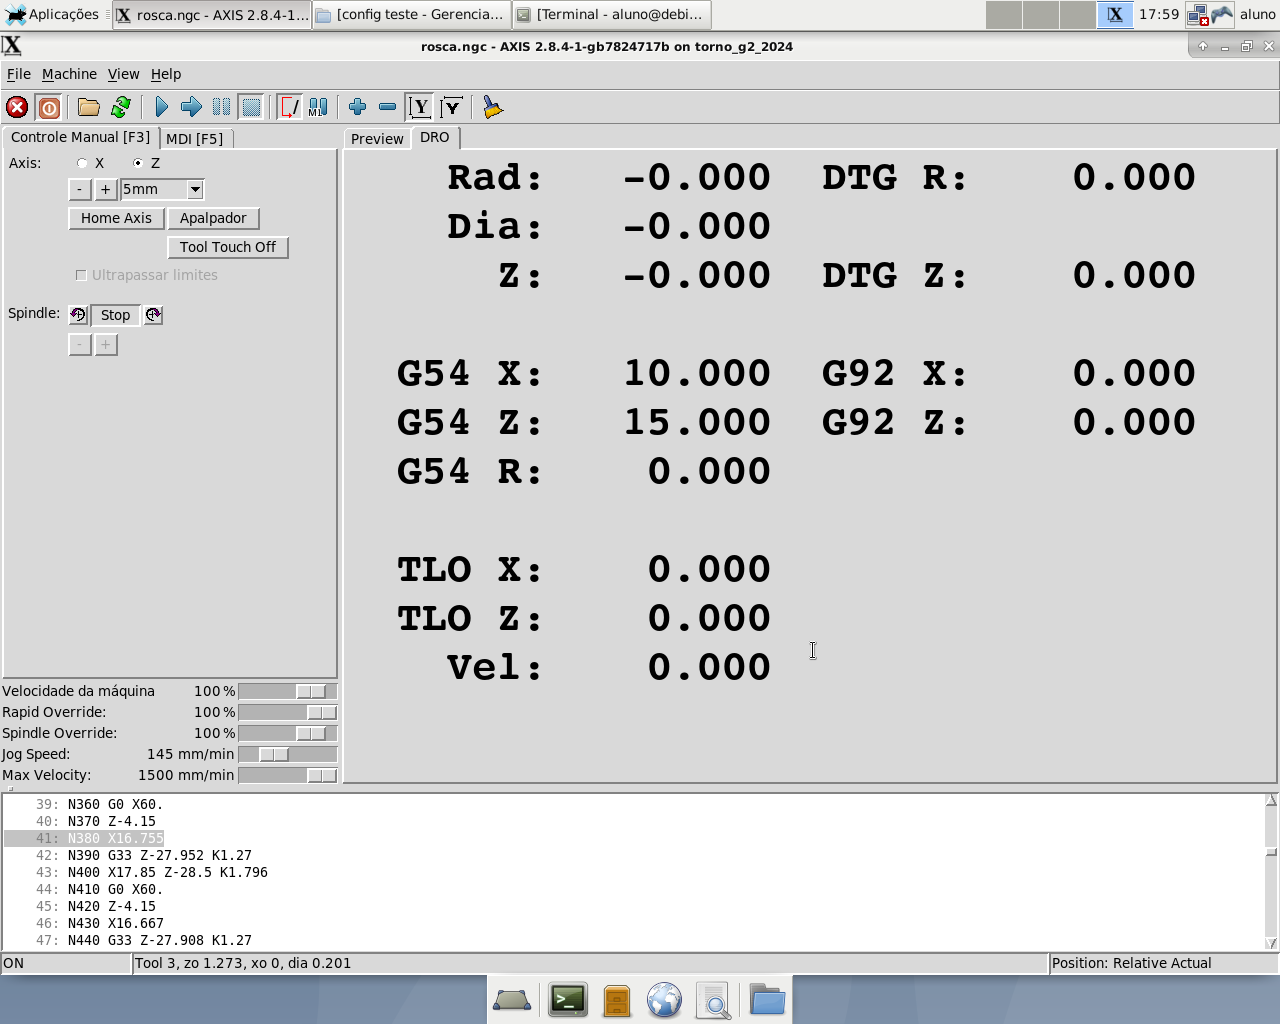
\includegraphics[width=0.95\textwidth]{imagens/configuracao_de_posicao.png}
    \end{center}
    \caption{}\label{fig:}
\end{figure}

\subsection{Testando o zero peça}

Se por alguma razão você estiver em dúvida sobre se o zero peça está definido no lugar certo (centro da face frontal do tarugo), você tem duas opções, refazer a calibração (recomendado), ou usar um comando no MDI para mandar a ferramenta para a coordenada (0, 0) definida em relação a G54 (tome muito cuidado).

Partindo de uma posição segura (ou seja, onde o movimento da ferramenta não tem chance de colidir com o tarugo), um comando como G54 G01 X0. Z0. F100. pode ser executado e se você definiu o zero peça corretamente, não devem haver problemas

\attention Se um procedimento como esse for executado, tenha certeza que você entende o que o comando que você digitar no MDI faz. Além disso, evite velocidades mais altas que a apresentada no exemplo.

\attention Fique atento, se a ferramenta colidir com o tarugo e não parar, esteja pronto para apertar o botão vermelho de emergência localizado na caixa de controle. É melhor ainda se houver outra pessoa pronta para apertar o botão enquanto você manuseia a máquina. 

\section{Executando código G}

Para executar um código G (contido em arquivos .ngc), você deve ter certeza de ter executado todos os passos necessárias anteriormente discutidos neste manual. Além disso, é importante verificar elementos mecânicos da máquina, listados a seguir:

\begin{itemize}
    \item Firmeza do acoplamento da placa de três castanhas ao eixo árvore 
    \item Afiação de todas as ferramentas que serão utilizadas durante a execução do programa 
    \item Distância da placa de três castanhas onde deve ser preso o tarugo, de modo que a peça planejada possa ser executada sem que hajam colisões com as chaves de fim de curso
    \item Firmeza do tarugo uma vez que a placa de castanhas tenha sido apertada
    \item Ajuste das velocidades de rotação do eixo árvore e dos motores de passo
\end{itemize}

É importante salientar que o passo de ajuste de velocidades dos motores de passo é fundamental para evitar avanços muito rápidos que podem lançar o tarugo ou as ferramentas para fora da máquina, o que pode gerar acidentes. Se não foi possível prender o tarugo de forma que sua face posterior toque a placa de castanhas, é quase certo que as velocidades terão de ser reduzidas. Para reduzir as velocidades programadas no código, podemos reduzir tanto a velocidade máxima da máquina, quanto definir um fator de redução (por exemplo se o slider for ajustado para 50\%, o programa roda na metade da velocidade programada no código) através da interface gráfica do LinuxCNC.

Com todas essas precauções tomadas, basta clicar no botão de executar, na interface gráfica do aplicativo. 

\attention Fique muito atento durante a execução de um programa, caso note que algo está dando errado aperte o botão de emergência imediatamente.

\attention Caso o programa pause no meio devido a uma seção no código que exige uma troca de ferramenta manual, troque a ferramenta, refaça os paços para a obtenção do zero peça, e então continue a execução do programa.  


\end{document}
